% ajupiter-c3-buffer.tex

\documentclass{standalone}
% jupiter-illustration-preamble.tex

\usepackage{tikz}
\usetikzlibrary{shapes, positioning, arrows.meta, calc, backgrounds, fit}

\def\hdist{1.8}
\def\vdist{2.0}
\tikzset{node distance = \vdist and \hdist}

\tikzset{every lower node part/.style = {red}}
\newcommand{\statesplit}[4]{% #1: state upper label; #2: state lower label; #3: position; #4
  \node (#4) [circle split, draw, minimum size = 6mm, text width = 10mm, align = center, #3, font = \Large]
  {
	$#1$
	\nodepart{lower}
	$#2$
  };
}

\newcommand{\transition}[4][]{% #2: start state; #3: end state; #4: transition label; #1: transition label position (optional)
  \draw[>=Stealth, ->] (#2) to node (#2to#3) [rectangle, draw, above = 2pt, sloped, #1, font = \small] {$#4$} (#3);
}

\newcommand{\set}[1]{\{#1\}}
\newcommand{\ins}[2]{\textsc{Ins}(#1,#2)}
\newcommand{\del}[2]{\textsc{Del}(#1,#2)}


\usetikzlibrary{chains}

\begin{document}
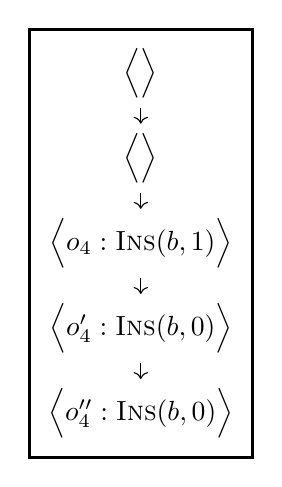
\begin{tikzpicture}[bg/.style = {rectangle, draw, very thick}, 
    start chain = going below,
    every on chain/.style = {join}, every join/.style = {->},
    node distance = 0.20cm]
  { \node (a) [on chain] {$\Big\langle \Big\rangle$};
    \node (b) [on chain] {$\Big\langle \Big\rangle$};
    \node (c) [on chain] {$\Big\langle o_4: \ins{b}{1} \Big\rangle$};
    \node (d) [on chain] {$\Big\langle o_4': \ins{b}{0} \Big\rangle$};
    \node (e) [on chain] {$\Big\langle o_4'': \ins{b}{0} \Big\rangle$};
  }

  \node () [fit = (a) (e), bg] {};
\end{tikzpicture}
\end{document}
